\begin{enumerate}[label=\thesection.\arabic*.,ref=\thesection.\theenumi]
\numberwithin{equation}{enumi}
\item Plot the polar plot of 
\begin{align}
G(s) = \frac{100(s+5)}{s(s+3)(s^2+4)}. 
\end{align}

\solution
The following python code generates the polar plot in Fig.   \ref{fig:ee18btech11042_polarplot}

\begin{lstlisting}
codes/ee18btech11042.py
\end{lstlisting}

\begin{figure}[!ht]
\centering
  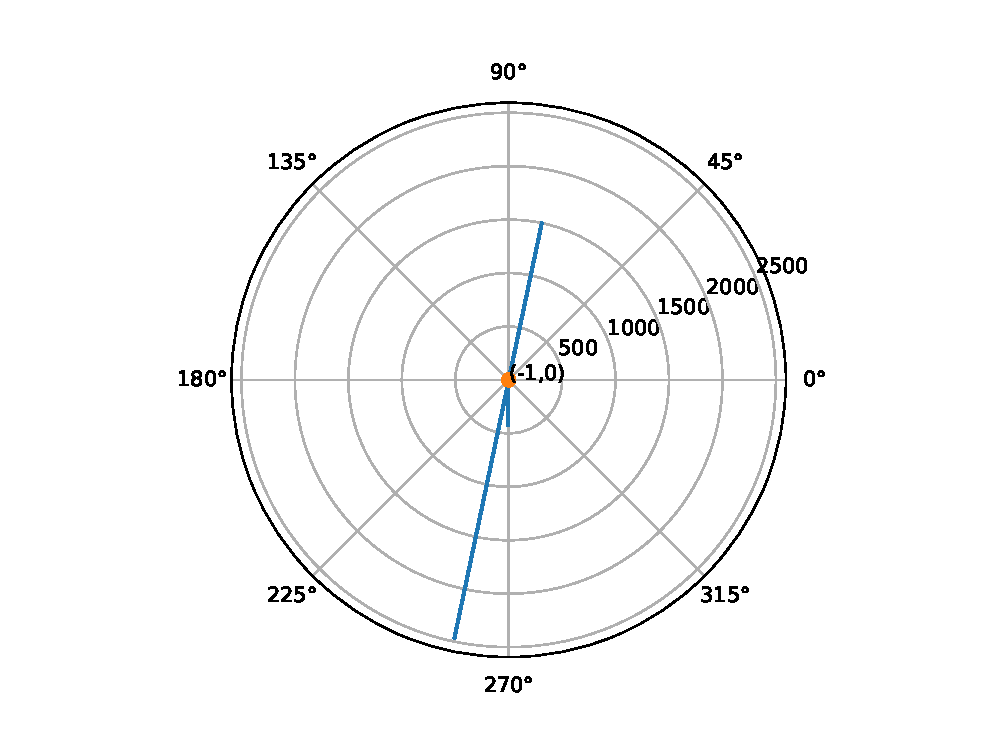
\includegraphics[width=\columnwidth]{./figs/ee18btech11042.eps}
\caption{}
  \label{fig:ee18btech11042_polarplot}
\end{figure}

Since (-1,0) is on the  polar plot, the  above system is  marginally stable.

\end{enumerate}


